\documentclass[8pt]{beamer}
\usefonttheme[onlymath]{serif}
\newcommand\bmale{\fontsize{6}{7.2}\selectfont}
\newcommand\male{\fontsize{8}{7.2}\selectfont}
\newcommand\normalne{\fontsize{10}{7.2}\selectfont}
\newcommand\duze{\fontsize{12}{7.2}\selectfont}
\setbeamertemplate{caption}{\raggedright\insertcaption\par}

\graphicspath{{commons/}}

 \AtBeginSection[]{
   \begin{frame}
   \vfill
 \centering
   \begin{beamercolorbox}[sep=8pt,center,shadow=true,rounded=true]{title}
     \usebeamerfont{title}\insertsectionhead\par%
   \end{beamercolorbox}
   \vfill
   \end{frame}
 }

\mode<presentation>
{
  \usetheme{CambridgeUS}
  \usecolortheme{beaver}
}
\usepackage{tikz}
\usetikzlibrary{shapes,arrows,positioning}
\tikzstyle{block} = [rectangle, draw, fill=blue!20, rounded corners, align = center, minimum height=2.5cm, minimum width=4cm]
\tikzstyle{line} = [draw, thin, ->, >=stealth]
\tikzstyle{cloud} = [draw, ellipse,fill=red!20, node distance=3cm,    minimum height=2em]

\usepackage{pgfplots}
\usepackage{ulem}
\usepackage{tabto}
\usepackage[]{algorithm2e}
\usepackage{bm}
\usepackage{lmodern}
\usepackage[T1]{fontenc}
\usepackage[polish]{babel}
\usepackage[utf8]{inputenc}
\usepackage{pgfplots}
\usepackage{textcomp}

\DeclareMathOperator*{\argmin}{argmin}
\DeclareMathOperator*{\argmax}{argmax}
\selectlanguage{polish}

\title[Kraków, 2018] % (optional, use only with long paper titles)
{Katedra Systemów Transportowych}

\subtitle
{Mobilność}

\author[dr in\.z. Rafa\l{} Kucharski] % (optional, use only with lots of authors)
{dr in\.z. Rafa\l{} Kucharski\inst{1}}

\institute[] % (optional, but mostly needed)
{
  \inst{1}%
  Katedra System\'{o}w Transportowych\\
  Politechnika Krakowska
 }


\date[KST, L-2, WIL, PK] % (optional, should be abbreviation of conference name)
{Krak\'{o}w, 2018}

\pgfdeclareimage[height=1cm]{university-logo}{commons/ZSK}
 \logo{\pgfuseimage{university-logo}}

\AtBeginSubsection[]
%{
%  \begin{frame}<beamer>{Outline}
%    \tableofcontents[currentsection,currentsubsection]
%  \end{frame}
%}
%\beamerdefaultoverlayspecification{<+->}


\begin{document}

\begin{frame}
  \titlepage
\end{frame}

\begin{frame}{Mobilność}{Definicje}

\begin{block}{Natężenie ruchu} Liczba pojazdów przejeżdżająca przez dany odcinek drogi w określonym czasie, \\ np. \textit{2 000 pojazdów na godzinę szczytu na kierunek w Alejach (Jubilat) }
\end{block}
\begin{block}{Potok pasażerski} Liczba pasażerów używających pojazdów komunikacji zbiorowej na danym odcinku w danym czasie, \\ np. \textit{18 000 pasażerów na kierunek pomiędzy stacją metra Centrum a Świętokrzyska w Warszawie w godzinie szczytu.}
\end{block}
\begin{block}{Czas przejazdu} Średni czas przejazdu odcinka (miedzy kolejnymi skrzyżowaniami, lub przystankami) lub relacji skrętnej (od dołączenia do kolejki do opuszczenia tarczy) w godzinie szczytu, np. \textit{15 minut pomiędzy przystankiem Politechnika a Nowy Kleparz o godzinie 16:15}
\end{block}
\end{frame}

\begin{frame}{Mobilność}{Definicje}

\begin{block}{Podróż}\begin{itemize}
\item rano z domu po bułki
\item z domu do pracy
\item z pracy na spotkanie
\item ze szkoły na gimnastykę
\item z pracy po dzieci z przedszkola
\item \dots
\end{itemize}
\end{block}
\begin{alertblock}{Mobilność} 
Potrzeba użytkowników (klientów) systemu transportowego przemieszczania się: \\\textbf{znalezienia się w innym miejscu przy jak najmniejszej uciążliwości}.
\end{alertblock}
Podstawowa przyczyna dla której potrzebne są systemy transportowe (podaż).

\end{frame}

\begin{frame}{Aktywności}{}
\begin{block}{Aktywność}
Przebywanie w określonym miejscu przez pewien okres czasu w związku z realizacją potrzeby.
\end{block}
Podstawowe aktywności:
\begin{itemize}
\item \textbf{DOM }(sen, rodzina, posiłki, zabawa, odpoczynek, wizyty, \dots)
\item \textbf{PRACA}
\item \textbf{SZKOŁA}
\\ oraz
\item zakupy
\item sprawy urzędowe
\item rozrywka
\item sport
\item wizyta
\item jedzenie
\item odwożenie, odprowadzanie
\item \dots
\end{itemize}

\end{frame}


\begin{frame}{Łańcuch}{Dobowy Łańcuch Aktywności}
\begin{block}{Łańcuch aktywności}
Sekwencja aktywności realizowanych przed daną osobę w ciągu doby
\end{block}
\begin{figure}
\begin{center}
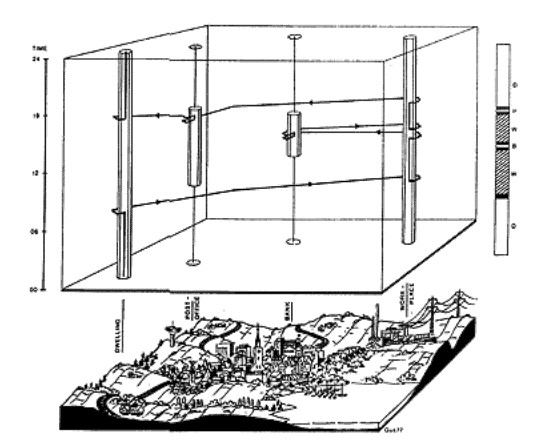
\includegraphics[height=5cm]{cylinder}
 \end{center}
 \caption{\small Cylinder czasoprzestrzenny}
 \end{figure}
\end{frame}


\begin{frame}{Łańcuchy podróży}
Łańcuch zazwyczaj kończy i zaczyna się w domu.
\begin{block}{Podstawowe łańcuchy trójelementowe}
\begin{itemize}
\item \texttt{Dom -> Praca -> Dom} (pracujący)
\item \texttt{Dom -> Szkoła -> Dom} (uczniowie)
\item \texttt{Dom -> Zakupy -> Dom} (bezrobotni, emeryci, niepracujący, urlop, itp.)
\end{itemize}
\end{block}
\begin{block}{Dodatkowa aktywność po podstawowej}
\begin{itemize}
\item \texttt{Dom -> Praca -> Zakupy -> Dom} 
\item \texttt{Dom -> Szkoła -> Rozrywka -> Dom}
\item \texttt{Dom -> Lekarz -> Odbieranie -> Dom} 
\end{itemize}
\end{block}
\begin{block}{Dodatkowa aktywność przed podstawową}
\begin{itemize}
\item \texttt{Dom -> Odwożenie -> Praca -> Zakupy -> Dom} 
\item \texttt{Dom -> Sport -> Szkoła -> Dom}
\item \texttt{Dom -> Odwożenie -> Lekarz -> Dom} 
\end{itemize}
\end{block}
\end{frame}

\begin{frame}{Liczność łańcuchów (Poznań 2010)}
\begin{table}[]
\begin{tabular}{l|l|l}
łańcuch & liczba podróży & udział \\ \hline \pause
DPD   & 5342 & 36.46\% \\ \pause
DSD   & 2382 & 16.26\% \\ \pause
DID   & 2032 & 13.87\% \\ \pause
DUD   & 1031 & 7.04\%  \\ \pause
DPDID & 347  & 2.37\%  \\ \pause
DPDUD & 211  & 1.44\%  \\ \pause
DSDID & 181  & 1.24\%  \\ \pause
DIDID & 178  & 1.21\%  \\ \pause
DIID  & 156  & 1.06\%  \\ \pause
DPID  & 149  & 1.02\%  \\ \pause
DPUD  & 96   & 0.66\% \\ \hline
\end{tabular}
\end{table}
\end{frame}




\begin{frame}{Macierz motywacji podróży}
\begin{figure}
\begin{center}
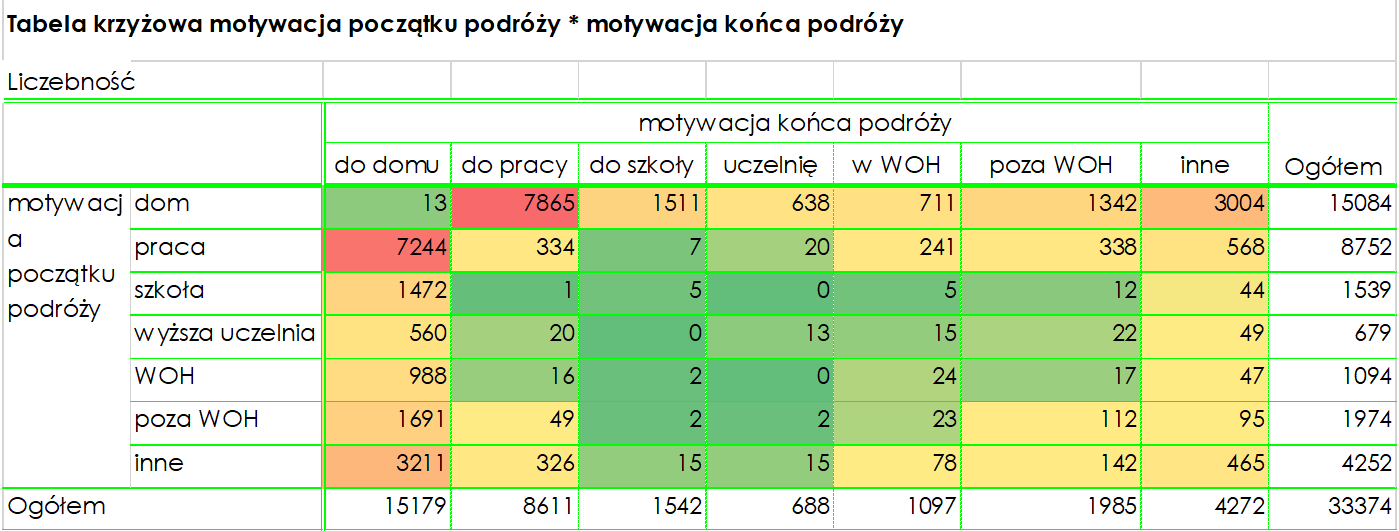
\includegraphics[height=4.5cm]{motywacje}
 \end{center}
 \caption{\small WBR 2015}
 \end{figure} 
\end{frame}

\section{Doba - aktywnosci i podroze}
\begin{frame}{Aktywnosci}
\begin{figure}
\begin{center}
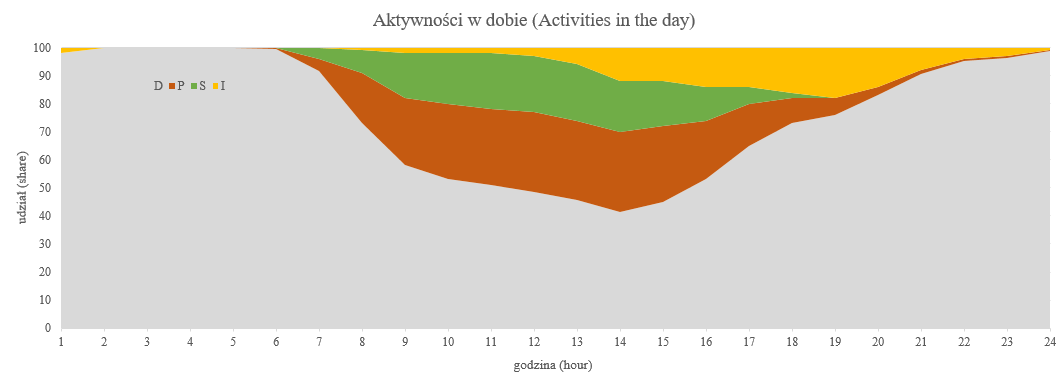
\includegraphics[width=0.95\textwidth]{act}
 \end{center}
 \end{figure} 
\end{frame}

\begin{frame}{Rozkład dobowy podróży}
\begin{figure}
\begin{center}
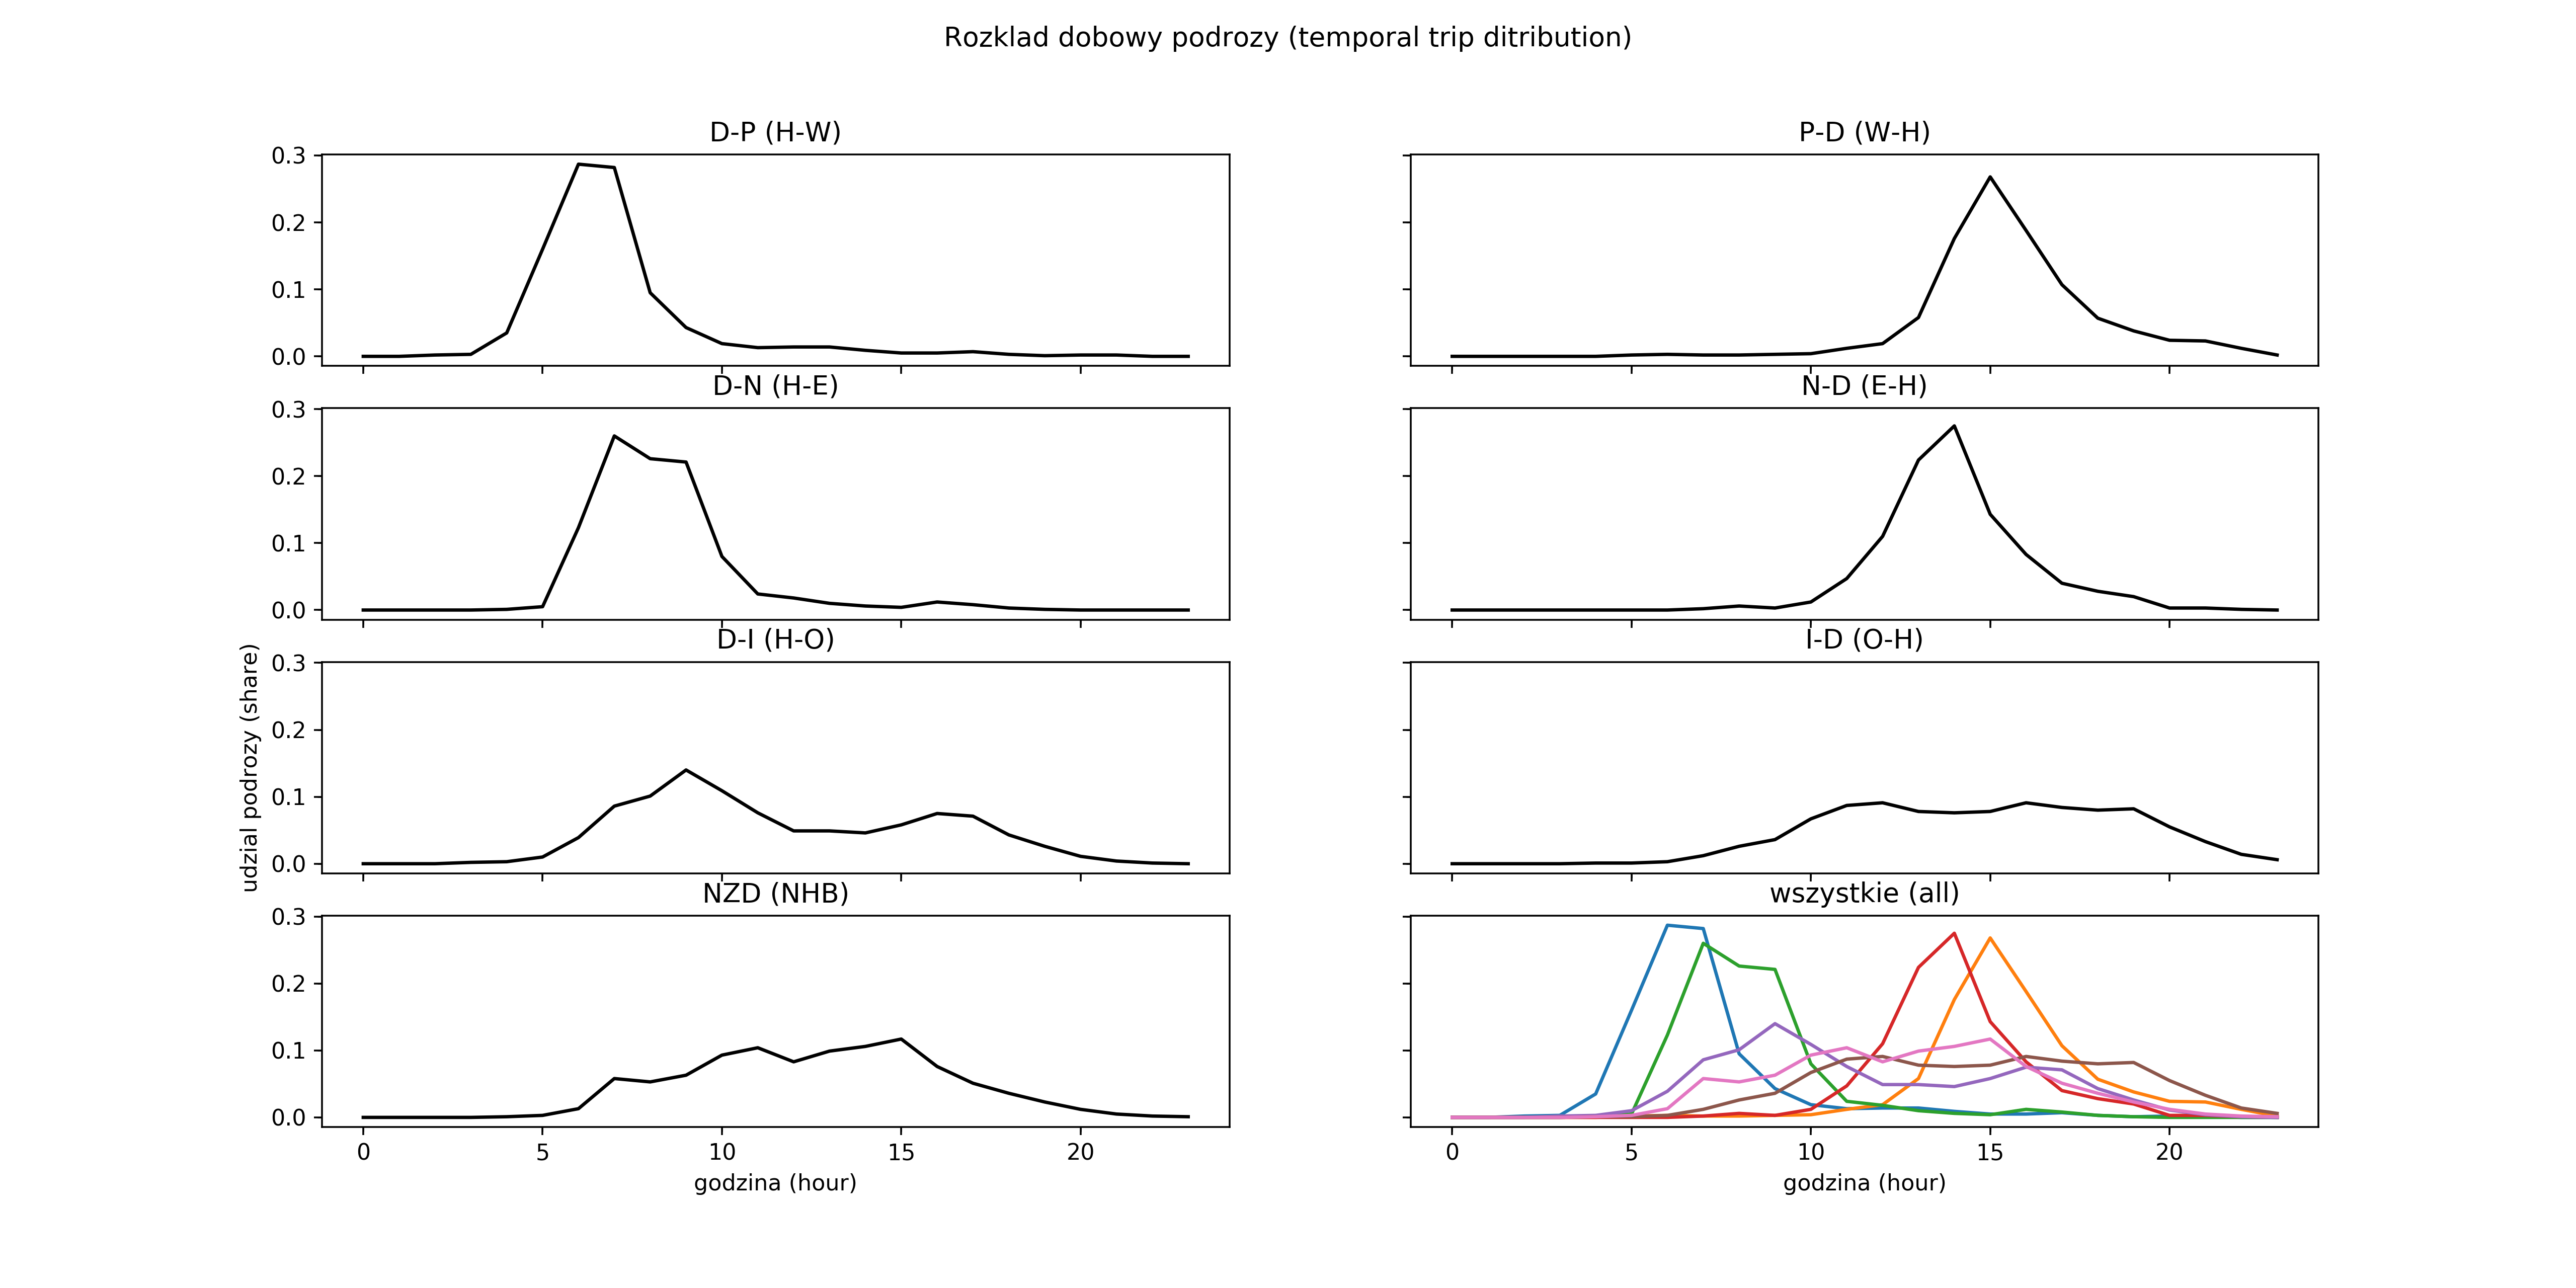
\includegraphics[width=1.1\textwidth]{dobowy}
 \end{center}
 \end{figure} 
\end{frame}

\begin{frame}{Rozkład dobowy podróży}
\begin{figure}
\begin{center}
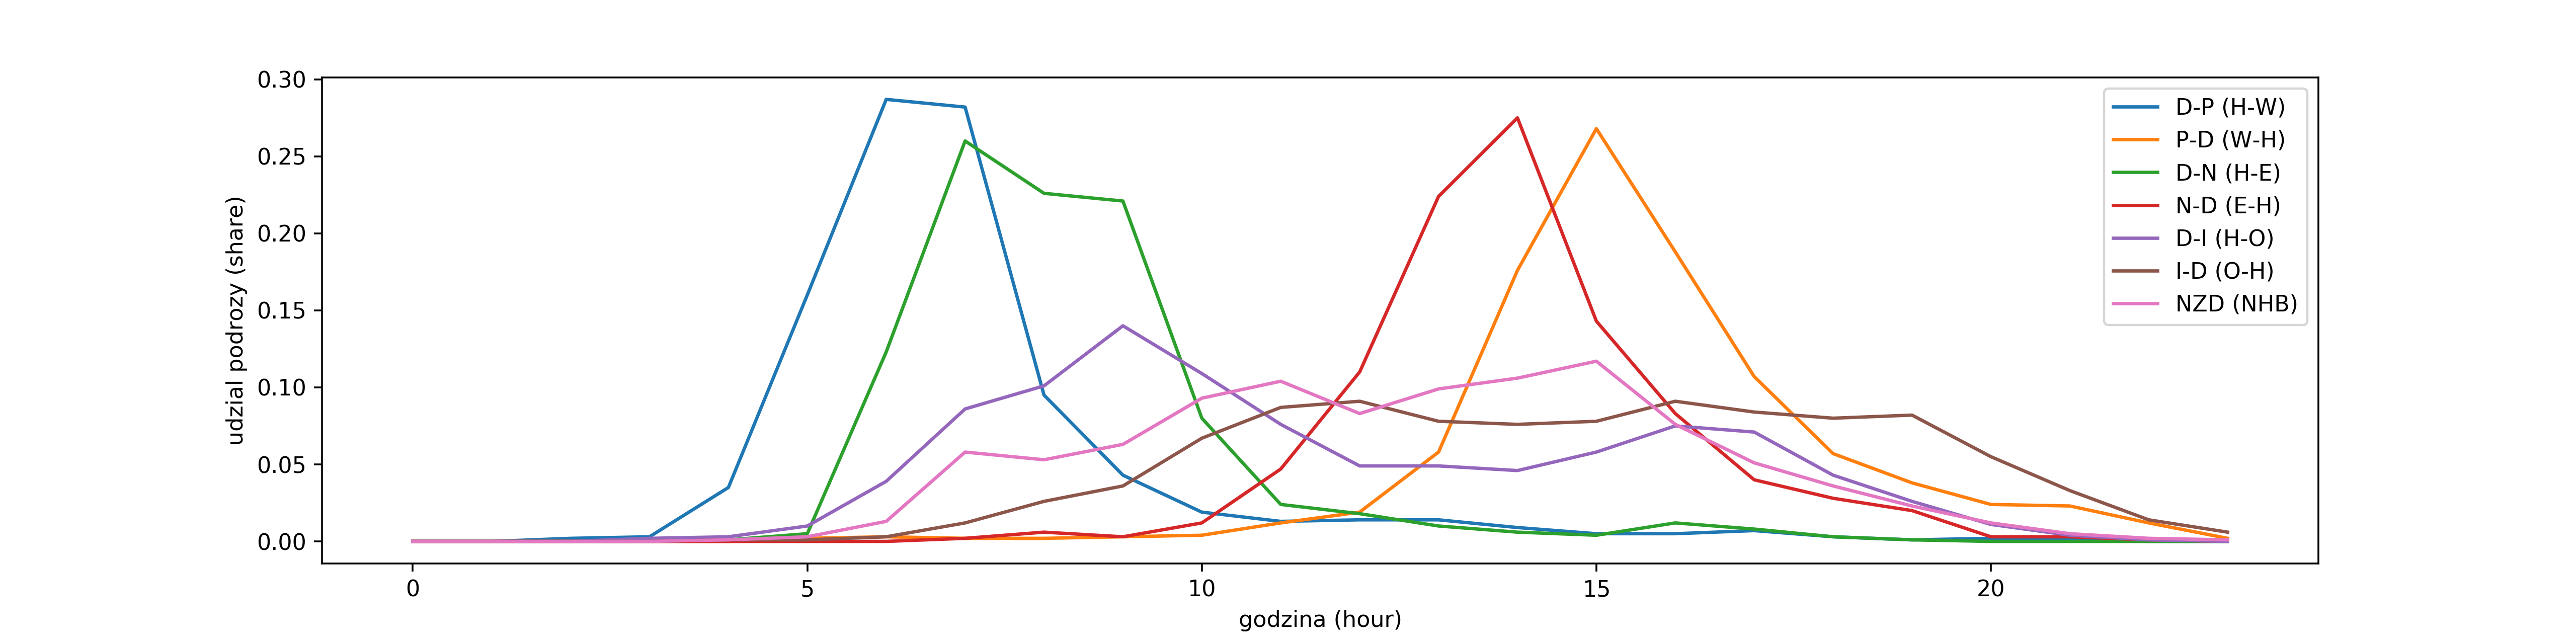
\includegraphics[width=1.1\textwidth]{all}
 \end{center}
 \end{figure} 
\end{frame}

\begin{frame}{Rozkład dobowy podróży}
\begin{figure}
\begin{center}
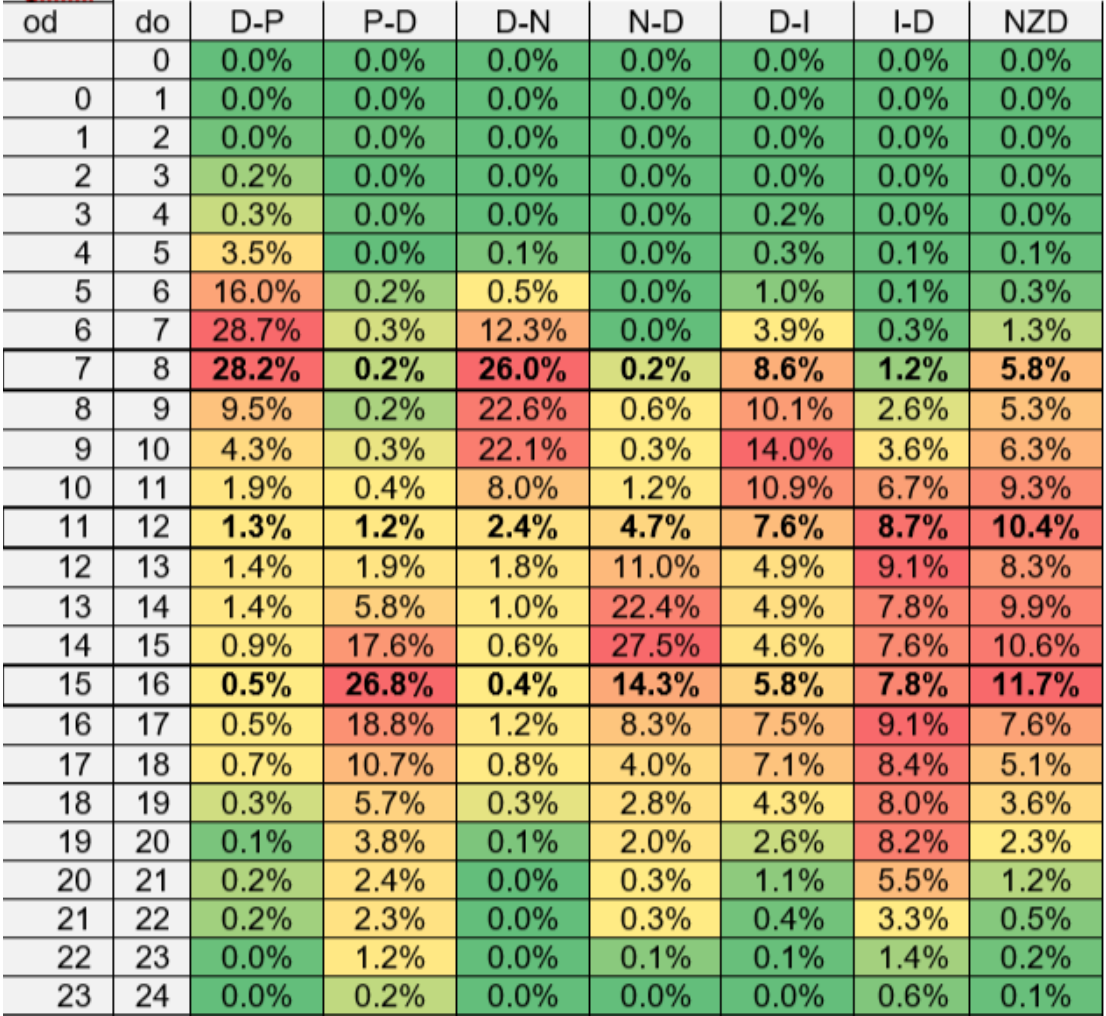
\includegraphics[width=0.55\textwidth]{kolorowe}
 \end{center}
 \end{figure} 
\end{frame}

\section{Model 4 stadiowy}
\begin{frame}{Model 4 stadiowy}{Wprowadzenie}
\begin{itemize}
\item analityczny
\item zgodny z KBR
\item czytelny
\item powtarzalny
\item wartości średnie (oczekiwane)
\item opisuje podróże (nie łańcuchy)
\end{itemize}
\end{frame}


\begin{frame}{Model 4 stadiowy}{opis}
\begin{table}[]
\begin{tabular}{l|c|c|c|c}
1 & \textbf{czy?/jak często?} &  produkcja i atrakcja rejonów & $q_o$, $q_d$ & \textbf{generacja podróży}\\ \hline 
2 & \textbf{dokąd?} &  więźba ruchu & $q_{od}$ & \textbf{grawitacja}\\ \hline 
3 & \textbf{czym?} &  udziały środków transportu  & $p_{od}$ & \textbf{wybór środka transportu}\\ \hline 
4 & \textbf{którędy?} &  obciążenia ścieżek & $q_a$ & \textbf{wybór trasy}\\ \hline 
\end{tabular}
\end{table}
\end{frame}


\begin{frame}{Model 4 stadiowy}
\begin{enumerate}
\item Na etapie \textbf{generacji ruchu} określamy liczbę podróży rozpoczynanych $q_o$ i kończonych $q_d$ w każdym rejonie używając formuł generacji zgodnie z zagospodarowaniem (zmienne rejonu $X_o$) i parametrami określonymi w KBR.
\item Na etapie \textbf{wyboru celu podróży} określamy liczbę podróży między rejonami $q_{od}$ na podstawie: 
\begin{itemize}
\item produkcji w źródle $q_o$, 
\item atrakcji u celu $q_d$
\item odległości pomiędzy rejonami (koszt $c_{od}$, lub czas $t_{od}$
\end{itemize}
\item Na etapie \textbf{wyboru środka transportu} dla każdej pary rejonów określamy prawdopodobieństwa $p_{od}$ wyboru każdego z rozważanych środków transportu:
\begin{itemize}
\item pieszo, \item komunikacją zbiorową, \item samochodem, \item ....
\end{itemize}
\item Na etapie \textbf{wyboru trasy} dla każdej pary źródło cel określ optymalną trasę: pieszą, komunikacją zbiorową, samochodem.

\end{enumerate}
\begin{equation}
\lbrace q_o, q_d \rbrace \rightarrow q_{od} \rightarrow q_{od} \times p_{m} \rightarrow q_a
\end{equation}
\end{frame}

\section{Generacja Ruchu}
\begin{frame}{Generacja ruchu}{Ujęcie statystyczne}
\begin{block}{Produkcja}
Liczba podrózy rozpoczynanych w danym okresie czasu w danym obszarze w danej motywacji. \\
np. \textit{Liczba podróży rozpoczynanych w dobie na Osiedlu Kościuszkowskim z domu do pracy}
\end{block}

\begin{block}{Atrakcja}
Liczba podrózy kończonych w danym okresie czasu w danym obszarze w danej motywacji. \\
np. \textit{Liczba podróży kończonych w dobie na Politechnice Krakowskiej z domu na uczelnię.}
\end{block}

\begin{block}{Ruchliwość}
Średnia liczba podrózy wykonywana przez osobę w dobie.
\end{block}
\begin{block}{Liczba podróży}
Najogólniej - ruchliwość razy liczba mieszkańców \\
$ T = \alpha \times LM_i$
\end{block}
\end{frame}



\begin{frame}{Czas wykonywania aktywności}
%\pgfmathdeclarefunction{gauss}{3}{%
% \pgfmathparse{#3/(#2*sqrt(2*pi))*exp(-((x-#1)^2)/(2*#2^2))}%
%}
%\begin{center}
%
%\begin{tikzpicture}
%\begin{axis}[ylabel=licznosc,xlabel=godzina, every axis plot post/.append style={
%  mark=none,domain=6:22,samples=50,smooth}, % All plots: from -2:2, 50 samples, smooth, no marks
%  axis x line*=bottom, % no box around the plot, only x and y axis
%  axis y line*=left, % the * suppresses the arrow tips
%  enlargelimits=upper]; % extend the axes a bit to the right and top
%  \addplot+[red] {gauss(6,2,1)};
%  \addplot+[red] {gauss(22,1.5,0.75)};
%  \addplot+[blue] {gauss(12,2.5,1)};
%  \addplot+[green] {gauss(11,2,0.5)};
%  \addplot+[brown] {gauss(13,1.5,0.3)};
%  \addplot+[pink] {gauss(16,3,0.5)};
%  \addlegendentry{Dom};
%  \addlegendentry{Dom};
%  \addlegendentry{Praca};
%  \addlegendentry{Szkoła};
%  \addlegendentry{Uczelnia};
%   \addlegendentry{Inne};\end{axis}
%\end{tikzpicture}
%\end{center}
\end{frame}


\section{Wybór celu podróży}
\begin{frame}{Wybór celu podróży}
\begin{block}{Sytuacja}
Wiemy gdzie i ile podróży rozpoczyna się (generacja) i kończy (atrakcja) \\
\alert{Nie wiemy} jakie to są podróże, nie wiemy jak początki łączą się z końcami.
\end{block}
\begin{block}{Wybór}
Podróżny:
\begin{itemize}
 \item jest w określonym miejscu (początek) 
 \item z określoną potrzebą (kolejną aktywnością w łańcuchu) 
 \item podejmuje decyzję gdzie zaspokoi potrzebę - wybiera koniec podróży
 \end{itemize} 
 \end{block}
\end{frame}

\begin{frame}{Wybór celu podróży}{Przykład}
Cztery rejony (1-4) generują podróże, w sumie 1000 podróży \\
które mogą być zaspokojone w dwóch rejonach, bliższym nr 5 i dalszym nr 6.
\begin{center}
\begin{minipage}{0.65\textwidth}
        
\begin{tikzpicture}[darkstyle/.style={circle,draw,fill=gray!40,minimum size=10}]

       \node [darkstyle]  (1) at (4,1) {3}; 
       \node [darkstyle]  (2) at (6,3) {2};
       \node [darkstyle]  (3) at (4,3) {1};
       \node [darkstyle]  (4) at (6,1) {4};
       \node [style={rectangle,draw,fill=gray!10,minimum size=20}]  (5) at (5,2) {5};
       \node [style={rectangle,draw,fill=gray!10,minimum size=20}]   (6) at (0,2) {6};
\end{tikzpicture}
    \end{minipage}\hfill
    \begin{minipage}{0.25\textwidth}
     \begin{center}
\begin{tabular}{|c|c|c|}
\hline 
{$o,d$} & P & A \\ 
\hline 
1 & 100 & -  \\ 
\hline 
2 & 200 & -  \\ 
\hline 
3 & 300 & -  \\ 
\hline 
4 & 400 & -    \\ 
\hline 
5 & - & 200  \\ 
\hline 
6 & - & 800  \\ 
\hline
\end{tabular}
\end{center}   
    \end{minipage}
\end{center}

\end{frame}

\begin{frame}{Wybór celu podróży}{Przykład}
\begin{center}
\begin{minipage}{0.65\textwidth}
        
\begin{tikzpicture}[darkstyle/.style={circle,draw,fill=gray!40,minimum size=10}]

       \node [darkstyle]  (1) at (4,1) {3}; 
       \node [darkstyle]  (2) at (6,3) {2};
       \node [darkstyle]  (3) at (4,3) {1};
       \node [darkstyle]  (4) at (6,1) {4};
       \node [style={rectangle,draw,fill=gray!10,minimum size=20}]  (5) at (5,2) {5};
       \node [style={rectangle,draw,fill=gray!10,minimum size=20}]   (6) at (0,2) {6};
\end{tikzpicture}
    \end{minipage}\hfill
    \begin{minipage}{0.25\textwidth}
     \begin{center}
\begin{tabular}{|c|c|c|}
\hline 
{$o,d$} & P & A \\ 
\hline 
1 & 100 & -  \\ 
\hline 
2 & 200 & -  \\ 
\hline 
3 & 300 & -  \\ 
\hline 
4 & 400 & -    \\ 
\hline 
5 & - & 200  \\ 
\hline 
6 & - & 800  \\ 
\hline
\end{tabular}
\end{center}   
    \end{minipage}
\end{center}
\begin{block}{Podróże fakultatywne o dużym oporze przestrzeni} 
np. na zakupy do najbliższej Biedronki
\end{block}
\begin{center}
\begin{tabular}{|c|c|c|}
\hline 
{$o,d,$}& 5 & 6 \\ 
\hline 
1 & 90 & 10  \\ 
\hline 
2 & 200 & 0 \\ 
\hline 
3 & 270 & 30 \\ 
\hline 
4 & 400 & 0 \\ 
\hline 
\end{tabular} 
\end{center}
\end{frame}

\begin{frame}{Wybór celu podróży}{Przykład}
\begin{center}
\begin{minipage}{0.65\textwidth}
        
\begin{tikzpicture}[darkstyle/.style={circle,draw,fill=gray!40,minimum size=10}]

       \node [darkstyle]  (1) at (4,1) {3}; 
       \node [darkstyle]  (2) at (6,3) {2};
       \node [darkstyle]  (3) at (4,3) {1};
       \node [darkstyle]  (4) at (6,1) {4};
       \node [style={rectangle,draw,fill=gray!10,minimum size=20}]  (5) at (5,2) {5};
       \node [style={rectangle,draw,fill=gray!10,minimum size=20}]   (6) at (0,2) {6};
\end{tikzpicture}
    \end{minipage}\hfill
    \begin{minipage}{0.25\textwidth}
     \begin{center}
\begin{tabular}{|c|c|c|}
\hline 
{$o,d$} & P & A \\ 
\hline 
1 & 100 & -  \\ 
\hline 
2 & 200 & -  \\ 
\hline 
3 & 300 & -  \\ 
\hline 
4 & 400 & -    \\ 
\hline 
5 & - & 200  \\ 
\hline 
6 & - & 800  \\ 
\hline
\end{tabular}
\end{center}   
    \end{minipage}
\end{center}
\begin{block}{Podróże fakultatywne o istotnej atrakcyjności celu podróży} 
np. do galerii handlowej przy dużej różnicy oferty (uwzględnione w atrakcji)
\end{block}
\begin{center}
\begin{tabular}{|c|c|c|}
\hline 
{$o,d,$}& 5 & 6 \\ 
\hline 
1 & 20 & 80  \\ 
\hline 
2 & 40 & 160 \\ 
\hline 
3 & 60 & 240 \\ 
\hline 
4 & 80 & 320 \\ 
\hline 
\end{tabular} 
\end{center}
\end{frame}


\begin{frame}{Wybór celu podróży}{Przykład}
\begin{center}
\begin{minipage}{0.65\textwidth}
        
\begin{tikzpicture}[darkstyle/.style={circle,draw,fill=gray!40,minimum size=10}]

       \node [darkstyle]  (1) at (4,1) {3}; 
       \node [darkstyle]  (2) at (6,3) {2};
       \node [darkstyle]  (3) at (4,3) {1};
       \node [darkstyle]  (4) at (6,1) {4};
       \node [style={rectangle,draw,fill=gray!10,minimum size=20}]  (5) at (5,2) {5};
       \node [style={rectangle,draw,fill=gray!10,minimum size=20}]   (6) at (0,2) {6};
\end{tikzpicture}
    \end{minipage}\hfill
    \begin{minipage}{0.35\textwidth}
     \begin{center}
\begin{tabular}{|c|c|c|}
\hline 
{$o,d$} & P & A \\ 
\hline 
1 & 100 & -  \\ 
\hline 
2 & 200 & -  \\ 
\hline 
3 & 300 & -  \\ 
\hline 
4 & 400 & -    \\ 
\hline 
5 & - & 200 \alert{-> 800}  \\ 
\hline 
6 & - & 800 \alert{-> 200} \\ 
\hline
\end{tabular}
\end{center}   
    \end{minipage}
\end{center}
\begin{block}{Podróże obligatoryjne gdzie podaż zdążyła dopasować się do popytu} 
np. do przedszkola
\end{block}
\begin{center}
\begin{tabular}{|c|c|c|}
\hline 
{$o,d,$}& 5 & 6 \\ 
\hline 
1 & 80 & 20  \\ 
\hline 
2 & 1600 & 40 \\ 
\hline 
3 & 240 & 60 \\ 
\hline 
4 & 320 & 80 \\ 
\hline 
\end{tabular} 
\end{center}
\end{frame}

\begin{frame}{Wybór celu podróży}{Przykład}
\begin{center}
\begin{minipage}{0.65\textwidth}
        
\begin{tikzpicture}[darkstyle/.style={circle,draw,fill=gray!40,minimum size=10}]

       \node [darkstyle]  (1) at (4,1) {3}; 
       \node [darkstyle]  (2) at (6,3) {2};
       \node [darkstyle]  (3) at (4,3) {1};
       \node [darkstyle]  (4) at (6,1) {4};
       \node [style={rectangle,draw,fill=gray!10,minimum size=20}]  (5) at (5,2) {5};
       \node [style={rectangle,draw,fill=gray!10,minimum size=20}]   (6) at (0,2) {6};
\end{tikzpicture}
    \end{minipage}\hfill
    \begin{minipage}{0.25\textwidth}
     \begin{center}
\begin{tabular}{|c|c|c|}
\hline 
{$o,d$} & P & A \\ 
\hline 
1 & 100 & -  \\ 
\hline 
2 & 200 & -  \\ 
\hline 
3 & 300 & -  \\ 
\hline 
4 & 400 & -    \\ 
\hline 
5 & - & 200  \\ 
\hline 
6 & - & 800  \\ 
\hline
\end{tabular}
\end{center}   
    \end{minipage}
\end{center}
\begin{block}{Podróże obligatoryjne o ograniczone pojemności celu podróży} 
np. do pracy przy określonej liczbie miejsc pracy (górna granica liczby podróży)
\end{block}
\begin{center}
\begin{tabular}{|c|c|c|}
\hline 
{$o,d,$}& 5 & 6 \\ 
\hline 
1 & 20 & 80  \\ 
\hline 
2 & 40 & 160 \\ 
\hline 
3 & 60 & 240 \\ 
\hline 
4 & 80 & 320 \\ 
\hline 
\end{tabular} 
\end{center}
\end{frame}

\begin{frame}{Faktyczna struktura przemieszczeń}{Ujawniona np. w śladach telefonów komórkowych}
\begin{figure}
\begin{center}
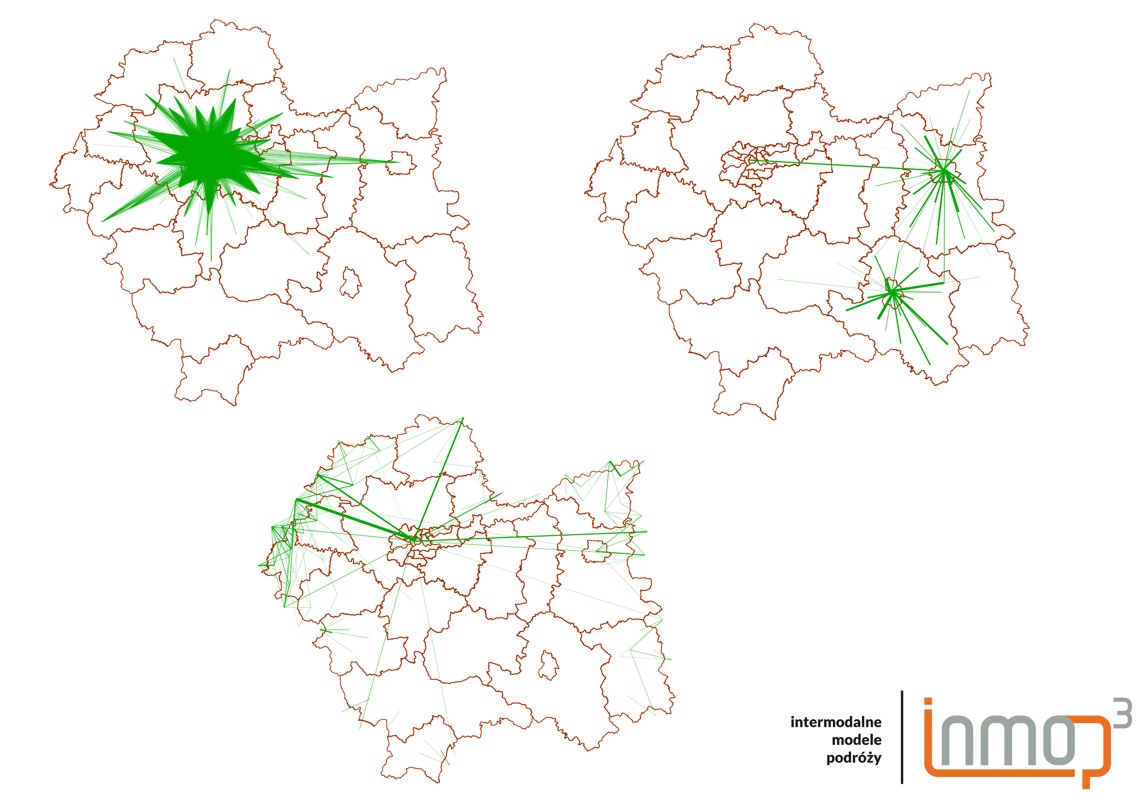
\includegraphics[height=7cm]{8}
 \end{center}
 \end{figure} 
 \end{frame}

\section{Popyt na nowej inwestycji}
\begin{frame}{Popyt na nowej inwestycji}
\begin{block}{Przykład}
Dzisiaj otwarto nową linie tramwajową w Krakowie. \\ Łączy ona Mistrzejowice, przez Park Wodny, Rondo Młyńskie, Wieczystą i dalej do Ronda Mogilskiego.\\
Pierwszego dnia po otwarciu kursem o 07:43 podróżuje \alert{100} pasażerów. \\
\alert{Skąd oni się wzięli?}
\end{block}
\end{frame}


\begin{frame}{Popyt na nowej inwestycji}{Przykład}
\begin{figure}
\begin{center}
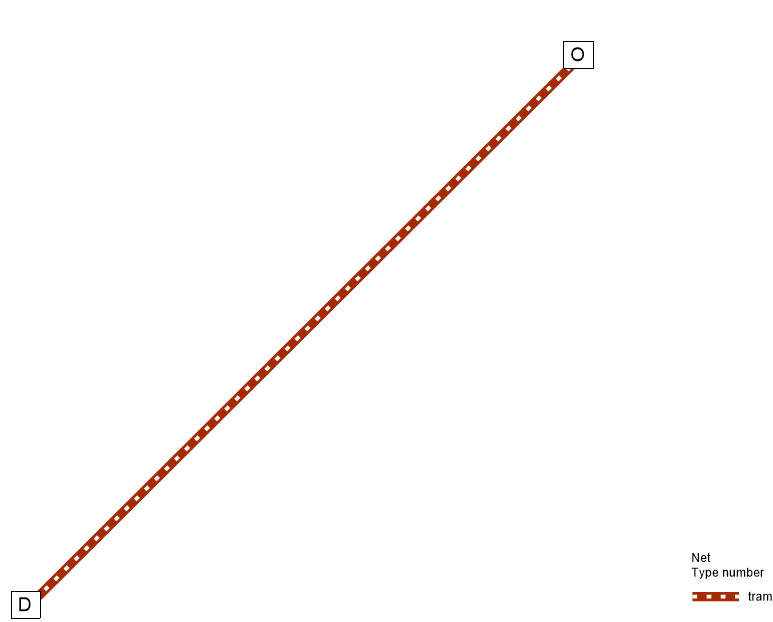
\includegraphics[height=7cm]{t1}
 \end{center}
 \end{figure}
\end{frame}


\begin{frame}{Popyt na nowej inwestycji}{Przykład}
\begin{figure}
\begin{center}
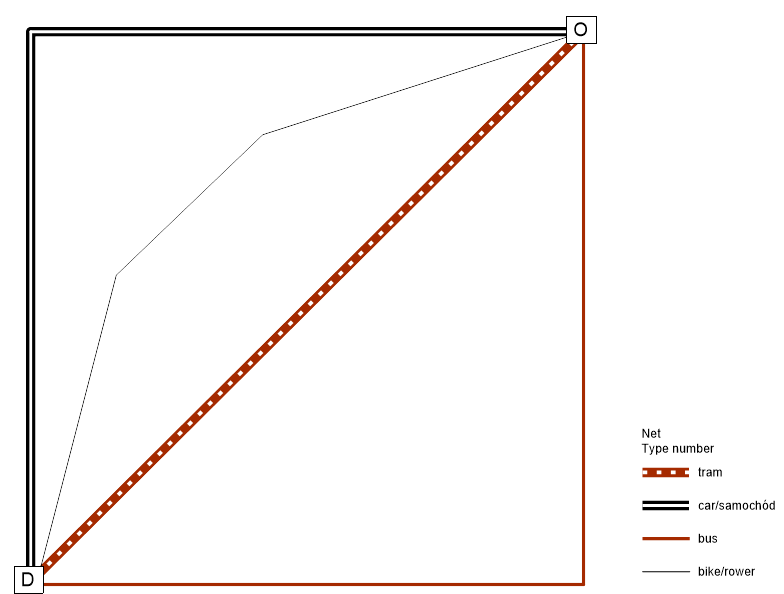
\includegraphics[height=7cm]{t2}
 \end{center}
 \end{figure}
\end{frame}


\begin{frame}{Popyt na nowej inwestycji}{Przykład}
\begin{figure}
\begin{center}
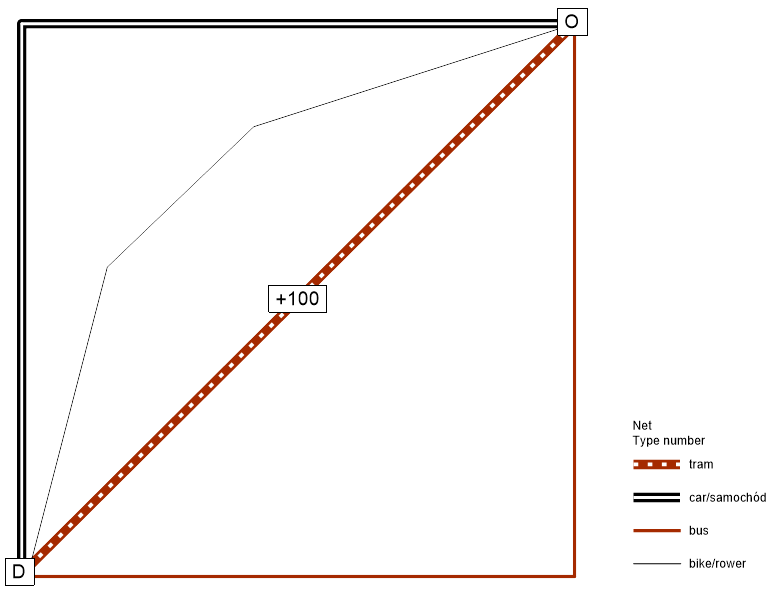
\includegraphics[height=7cm]{t3}
 \end{center}
 \end{figure}
\end{frame}

\begin{frame}{Popyt na nowej inwestycji}{Przykład}
\begin{figure}
\begin{center}
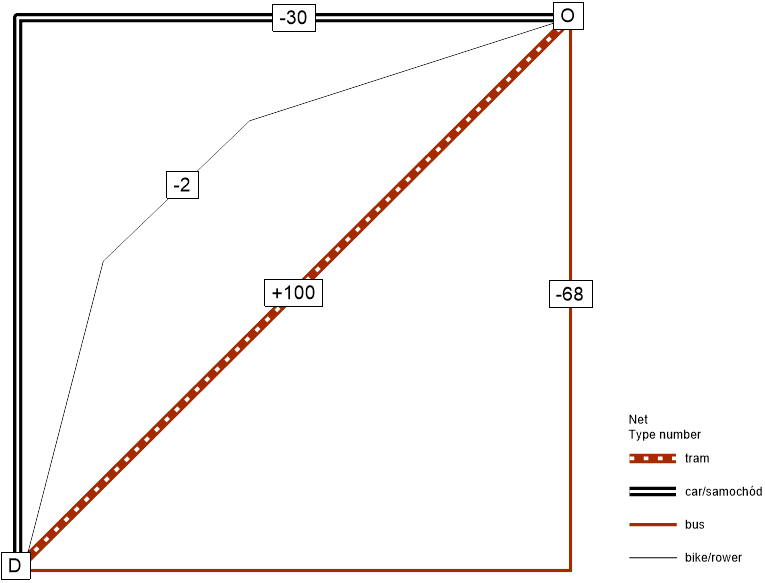
\includegraphics[height=7cm]{t4}
 \end{center}
 \end{figure}
\end{frame}

\section{Wybór trasy}
\begin{frame}{Wybór ścieżki w sieci drogowej}
Dla przedstawionej poniżej sieci drogowej określmy obciążenie (liczbę pojazdów $q_a$) na moście (odcinek przerywany) i wynikający z niego czasu przejazdu ($t_a$). Wartości w rejonach oznaczają liczbę pojazdów jaka w ciągu godziny szczytu porannego chce dojechać do celu podróży. Załóż, że wszystkie odcinki są równe i czas przejazdu każdego z nich w ruchu swobodnym wynosi 1 minutę.
\begin{enumerate}
\item załóż, że przepustowość wszystkich odcinków jest nieograniczona.
\item załóż, że przepustowość ($Q_a$) mostu (odcinek przerywany) wynosi 500 pojazdów na godzinę, pozostałe odcinki mają nieograniczoną przepustowość. Czas przejazdu oszacuj korzystając z funkcji: $t_a=t_a^0 \cdot (1+ (q_a / Q_a)^2)$. Podaj szacunkową wartość zbliżoną do warunków równowagi Wardop'a.
\end{enumerate}
\end{frame}



\begin{frame}{Wybór ścieżki w sieci}{przykład}
A: przepustowość wszystkich odcinków jest nieograniczona.
\begin{center}
\begin{tikzpicture}[darkstyle/.style={circle,draw,fill=gray!40,minimum size=20}]
\draw (6,4)--(6,2) ;
\draw (8,4)--(8,2) ;
\draw (10,4)--(10,2) ;
\draw (0,2)--(10,2) ;
\draw (0,2)--(0,0) ;
\draw (0,0)--(8,0) ;
\draw (8,0)--(8,2) ;
\draw (8,0)--(8,-2) ;
       \node [darkstyle]  (1) at (6,4) {1000}; 
       \node [darkstyle]  (2) at (8,4) {300};
       \node [darkstyle]  (3) at (10,4) {700};
       \node [style={circle,draw,fill=gray!10,minimum size=20}]  (1) at (8,-2) {Cel}; 
       \node [style={circle,draw,fill=gray!0,minimum size=1}]  (1) at (0,0) {}; 
       \node [style={circle,draw,fill=gray!0,minimum size=1}]  (1) at (2,0) {};
       \node [style={circle,draw,fill=gray!0,minimum size=1}]  (1) at (4,0) {};
       \node [style={circle,draw,fill=gray!0,minimum size=1}]  (1) at (6,0) {};   
       \node [style={circle,draw,fill=gray!0,minimum size=1}]  (1) at (8,0) {}; 
       \node [style={circle,draw,fill=gray!0,minimum size=1}]  (1) at (0,2) {}; 
       \node [style={circle,draw,fill=gray!0,minimum size=1}]  (1) at (2,2) {};
       \node [style={circle,draw,fill=gray!0,minimum size=1}]  (1) at (4,2) {};  
       \node [style={circle,draw,fill=gray!0,minimum size=1}]  (1) at (6,2) {}; 
       \node [style={circle,draw,fill=gray!0,minimum size=1}]  (1) at (8,2) {}; 
       \node [style={circle,draw,fill=gray!0,minimum size=1}]  (1) at (10,2) {}; 
       
       
\end{tikzpicture}
\end{center}
\end{frame}


\begin{frame}{Wybór ścieżki w sieci}{przykład}
B: przepustowość ($Q_a$) mostu (odcinek przerywany) wynosi 500 pojazdów na godzinę, pozostałe odcinki mają nieograniczoną przepustowość. Czas przejazdu oszacuj korzystając z funkcji: $t_a=t_a^0 \cdot (1+ (q_a / Q_a)^2)$. Podaj szacunkową wartość zbliżoną do warunków równowagi Wardop'a.
\begin{center}
\begin{tikzpicture}[darkstyle/.style={circle,draw,fill=gray!40,minimum size=20}]
\draw (6,4)--(6,2) ;
\draw (8,4)--(8,2) ;
\draw (10,4)--(10,2) ;
\draw (0,2)--(10,2) ;
\draw (0,2)--(0,0) ;
\draw (0,0)--(8,0) ;
\draw [thick, dashed] (8,0)--(8,2) ;
\draw (8,0)--(8,-1) ;
       \node [darkstyle]  (1) at (6,4) {1000}; 
       \node [darkstyle]  (2) at (8,4) {300};
       \node [darkstyle]  (3) at (10,4) {700};
       \node [style={circle,draw,fill=gray!10,minimum size=20}]  (1) at (8,-1) {Cel}; 
       \node [style={circle,draw,fill=gray!0,minimum size=1}]  (1) at (0,0) {}; 
       \node [style={circle,draw,fill=gray!0,minimum size=1}]  (1) at (2,0) {};
       \node [style={circle,draw,fill=gray!0,minimum size=1}]  (1) at (4,0) {};
       \node [style={circle,draw,fill=gray!0,minimum size=1}]  (1) at (6,0) {};   
       \node [style={circle,draw,fill=gray!0,minimum size=1}]  (1) at (8,0) {}; 
       \node [style={circle,draw,fill=gray!0,minimum size=1}]  (1) at (0,2) {}; 
       \node [style={circle,draw,fill=gray!0,minimum size=1}]  (1) at (2,2) {};
       \node [style={circle,draw,fill=gray!0,minimum size=1}]  (1) at (4,2) {};  
       \node [style={circle,draw,fill=gray!0,minimum size=1}]  (1) at (6,2) {}; 
       \node [style={circle,draw,fill=gray!0,minimum size=1}]  (1) at (8,2) {}; 
       \node [style={circle,draw,fill=gray!0,minimum size=1}]  (1) at (10,2) {}; 
       
       
\end{tikzpicture}
\end{center}
\end{frame}


\begin{frame}{Podsumowanie}{Dziękuję za uwagę}
Rafal Kucharski, rkucharski(at)pk.edu.pl
\end{frame}

\end{document}



